%   The formal model developed above can be used for the analysis of several systems. 
%  In the previous section, we introduced the formal model that allows regularly describing delivery guarantees and proposed necessary and sufficient conditions of~ exactly-once. In this section, we demonstrate how implementations of exactly-once in state-of-the-art distributed stream processing systems satisfy the necessary condition of~ exactly-once. 

\subsection{MillWheel}

 The $\Gamma$ is all possible streaming {\em records}. Dependency relation $D$ is defined using a graph of user-defined transformations. 
 To ensure fault tolerance,   MillWheel employs a {\em strong productions}~\cite{Akidau:2013:MFS:2536222.2536229}   mechanism that stores persistently input and output of operation for each new input item.
 Thus each streaming element is saved before it may influence other elements or operation states. 
 Recovery function $F$ resends all saved records in case of failure, and each operation deduplicates input that has been already processed.

The necessary condition of exactly-once from Theorem~\ref{necessary_conditions} claims that each element $s \in \Gamma$ obtained through a non-commutative operation must be persistently saved before any other element $b_{\tau} \in Cl_D(s)$ that depends on $s$ is released. Strong productions mechanism ensures that this condition is satisfied, i.e., if some element $b_\tau$ is released, it is guaranteed that its dependencies were released earlier (saved to persistent storage). The idea of this method is shown in Figure~\ref{millwheel}. It demonstrates that in MillWheel, all elements become recoverable, so there is no need to reprocess them again from an input item in case of failure. 

\begin{figure}[htbp]
  \centering
  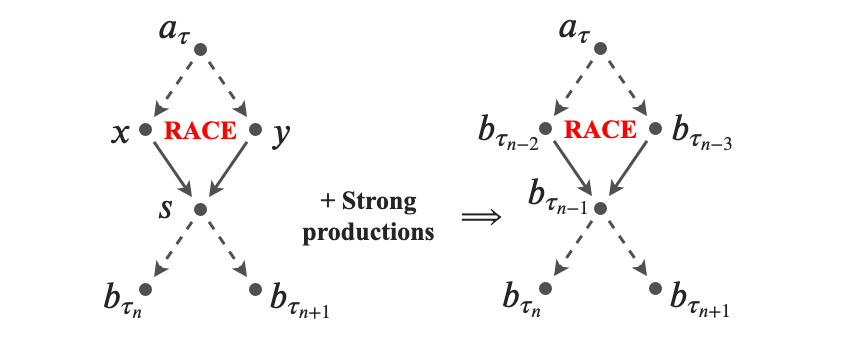
\includegraphics[width=0.48\textwidth]{Chapters/DeliveryGuarantees/pics/millwheel.png}
  \caption{Strong productions mechanism}
  \label{millwheel}
\end{figure}

Such behavior is also called {\em effective determinism}~\cite{akidau2018streaming} because computations become deterministic until the persistent storage is cleared. Strong productions method guarantees that even if many possible results of a non-commutative operation may be obtained due to races, only one of them is computed and saved. The price for such exactly-once enforcement is an overhead on external writes on each transformation in a physical graph.

\subsection{Spark streaming}

In Spark, the  $\Gamma$   is a set of all possible small collections of input items called  {\em RDD} records that are processed atomically.
Dependency relation on the power set of $\Gamma$ is also defined using a directed acyclic graph of user operations. 
Spark inherits main properties of batch processing systems:  each new stage of computations is started only after the previous one is completed and recovery function $F$ starts reprocessing of a micro-batch from the beginning in case of failure.

The condition for exactly-once from Theorem~\ref{necessary_conditions} is satisfied because all elements within the micro-batch are released atomically. Elements from various micro-batches can interact only through persistently stored state. 
Output elements that are ready to be delivered to the end-user must wait until the whole micro-batch is completely processed. 
Therefore, if two output elements $b_{\tau_1},b_{\tau_2} \in Cl_D(s)$ depend on a single item $s$, it is guaranteed that $\tau_1=\tau_2$. The illustration of this behavior is shown in Figure~\ref{spark_flink}. 
 
\begin{figure}[htbp]
  \centering
  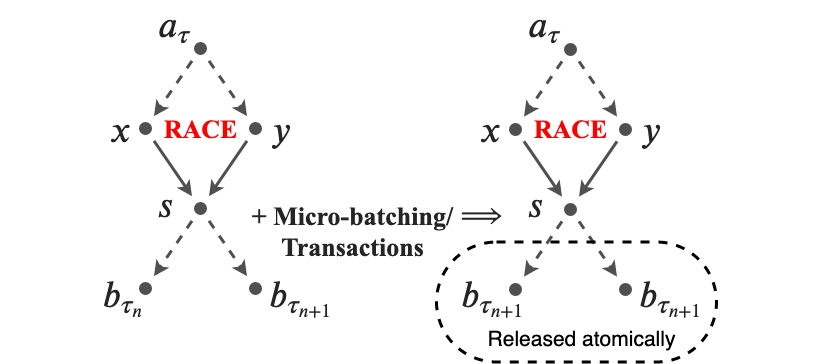
\includegraphics[width=0.48\textwidth]{Chapters/DeliveryGuarantees/pics/spark-flink.png}
  \caption{Micro-batching and transactional approach}
  \label{spark_flink}
\end{figure}
 
% Micro-batching technique ensures determinism as well. To the best of our knowledge, spark streaming is the only state-of-the-art stream processing system that provides for deterministic results. Another advantage of micro-batching is a high throughput~\cite{karimov2018benchmarking}. However, an architecture based on the processing of collections of buffered input elements makes it hard to achieve latency lower than several seconds~\cite{7530084, 7474816}. 

\subsection{Flink}

In Flink, the  $\Gamma$ is represented as all {\em StreamRecords}. Relation $D$ is defined in the form of a directed acyclic graph consisting of user operations. 
Flink periodically saves information needed for recovery by injecting particular elements called {\em checkpoints} into the input stream. 
Intervals  between checkpoints are called {\em epochs}. Checkpoints go through the same network channels as common elements and push all inverted dependencies of inputs through the system. 
Each operation prepares data to save independently at the moment of checkpoint arrival. Prepared data is committed to external storage when checkpoint passes through the whole data flow. Output elements are delivered to the end-user only after the commit. 
Recovery function $F$ reprocesses last non-complete epochs.

This mechanism ensures that all elements within an epoch are processed atomically and all interactions between elements from different epochs are possible only through persistent state. 
Hence, as it is shown in Figure~\ref{spark_flink},
 if two output elements $b_{\tau_1},b_{\tau_2} \in Cl_D(s)$ depend on a single item $s$, 
 it is guaranteed that $\tau_1=\tau_2$. 
This ensures that the necessary condition of exactly-once from Theorem~\ref{necessary_conditions} is satisfied. 
Such a method is quite similar to the micro-batching technique used in Spark. 
The differences are: elements are buffered after their processing is done and  multiple epochs can be processed simultaneously. 
%  These facts allow Flink to achieve lower latency in comparison with micro-batching, because at the end of an epoch, most of the elements which belong to this epoch, has already been processed.
